\documentclass[twoside,11pt]{article}

% Any additional packages needed should be included after jmlr2e.
% Note that jmlr2e.sty includes epsfig, amssymb, natbib and graphicx,
% and defines many common macros, such as 'proof' and 'example'.
%
% It also sets the bibliographystyle to plainnat; for more information on
% natbib citation styles, see the natbib documentation, a copy of which
% is archived at http://www.jmlr.org/format/natbib.pdf

\usepackage{jmlr2e}
\usepackage{amsmath}
\usepackage{caption}
\usepackage{mwe}
\usepackage{subcaption}

% Definitions of handy macros can go here

\newcommand{\dataset}{{\cal D}}
\newcommand{\fracpartial}[2]{\frac{\partial #1}{\partial  #2}}
\newcommand{\method}{{Deep MR}}

% Heading arguments are {volume}{year}{pages}{submitted}{published}{author-full-names}

\jmlrheading{1}{2000}{1-48}{4/00}{10/00}{Marina Meil\u{a} and Michael I. Jordan}

% Short headings should be running head and authors last names

\ShortHeadings{Deep Mendelian Randomization: Interrogating Genomic Deep Learning Models' Causal Knowledge}{Malina and Knowles}
\firstpageno{1}

\begin{document}

\title{Deep Mendelian Randomization: Identifying and Verifying Genomic Deep Learning Models' Causal Knowledge}

\author{\name Stephen Malina \email sdm2181@columbia.edu \\
       \AND
	\name Daniel Cizin \email todo@todo.edu \\
       \AND
       \name David A. Knowles \email dak2173@columbia.edu}
       

\editor{N/A}

\maketitle

\section{Introduction}
\begin{itemize}
	\item \textbf{Motivation}: interrogating genome-level causal relationships learned by multi-task sequence-to-function machine learning models.
	\item \textbf{Method summary}: Our method estimates causal effects for cause (`exposure') and effect (`outcome') feature pairs from a sequence-to-function model's predicted labels. It requires:
		\begin{itemize}
			\item A trained multi-task (classification or regression) model.
			\item Method for getting the model to output predictive means and standard errors or a full predictive distribution.
			\item Sample sequence inputs.
		\end{itemize}
	\item \textbf{Experiments summary}: To test our method, we conducted 3 experiments:
		\begin{enumerate}
			\item Simulation experiment
			\item BPNet (\cite{avsec2020base}) experiment
			\item DeepSEA (TODO) (\cite{zhou2015predicting}) experiment
		\end{enumerate}
	\item \textbf{Results summary}: our results suggest that backing out causal relationships from a sequence-to-function model is possible.
		\begin{itemize}
			\item \textbf{Simulation experiment}: good at recovering global relationships, even in presence of confounding (TODO: double-check after re-running). 
			\item \textbf{BPNet experiment}: recovers expected global effect pattern.
			\item \textbf{DeepSEA experiment}: TODO
		\end{itemize}
	\item \textbf{Related work}: 
	\begin{enumerate}
		\item Builds on genomic DL literature
		\item Leverage probabilistic DL model papers - MC dropout \& deep ensembles
		\item Complements interpretability work
	\end{enumerate} 
\end{itemize}

\section{Methods}%
\label{sec:methods}

\subsection{Algorithm}%
\label{sub:algorithm}
\begin{figure*}[htpb]
    \centering
    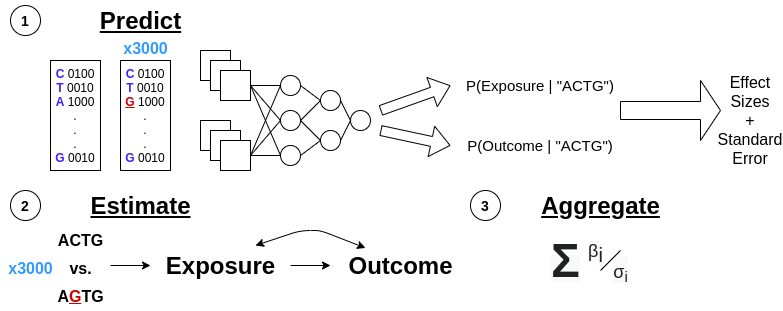
\includegraphics[width=.8\linewidth]{fig/model_overview.png}
    \vspace{-12pt}
    \caption{Graphical representation of \method's high-level steps combining \textit{in silico} mutagenesis and MR (see Section \ref{ssub:algo_overview}). \underline{Predict} corresponds to steps 1 through 4. \underline{Estimate} corresponds to step 5. \underline{Aggregate} corresponds to step 6}
    \vspace{-10pt}
    \label{fig:model_overview}
\end{figure*}

\paragraph{Inputs}%
\label{par:inputs}
\method\ takes a calibrated, trained model and a set of one-hot encoded sequences as input. In our case, the one-hot encoded sequence represents a sequence of nucleotides for the model to make predictions on.

\paragraph{Outputs}%
\label{par:outputs}
\method\ outputs local, sequence-specific causal effects and global, exposure-specific causal effects. 

\subsubsection{Overview}%
\method\ accomplishes its goal via the following procedure: 
\label{ssub:algo_overview}
\begin{enumerate}
    \item Randomly sample sequences to predict exposure and outcome values for ``reference sequences''.
    \item Perform \textit{saturation in-silico mutagenesis} for each reference sequence to generate \( (\text{sequence\ length} \times \text{alphabet\ size} - 1) \) mutated sequences per reference sequence.
    \item For each reference and set of mutated sequences, generate predictive means and standard errors for the reference and mutated sequences.
    \item Generate \( (\text{sequence length} \times \text{alphabet size} - 1) \) \textit{effect sizes} by subtracting each reference sequence's predictive mean from the corresponding mutated sequences' predictive means. Also, compute the standard errors of these differences.
    \item Estimate a per-exposure, per-sequence region causal effect by running MR on the effect sizes and their standard errors.
    \item Estimate overall per-exposure causal effects using a random effects meta-analysis.
\end{enumerate}

\subsubsection{Key Assumptions}%
\label{ssub:key_assumptions}
Devote a paragraph(s) to discussing the assumptions \method\ relies on and maybe 1 sentence just mentioning why we think the assumption is satisfied for each. These assumptions are:
\begin{itemize}
	\item Local linearity
	\item MR DAG faithfulness
	\item Model performance
		\begin{itemize}
			\item Accuracy upper bound and variant effect prediction warning
			\item Inherited biases
			\item Calibration (reference later section on dealing with this)
		\end{itemize}
\end{itemize}


\subsubsection{Components}%
\label{ssub:algo_components}
\paragraph{Mendelian Randomization}%
\label{par:mendelian_randomization}
\begin{itemize}
	\item Introduce MR assumptions
	\item Discuss method we choose and its additional assumptions / features (what assumptions it allows us to weaken)
\end{itemize}

\paragraph{Calibrated probabilistic model}%
\label{par:calibrated_probabilistic_model}
\begin{itemize}
	\item We use deep learning models in all of our experiments
	\item Discuss two methods we use for making DL models probabilistic
	\item Reference how we calibrate them (\cite{kuleshov2018accurate})
\end{itemize}

\section{Experiments}%
\label{sec:experiments}
In which we describe the three experiments we conducted and their results.

\subsection{Simulation}%
\label{sub:simulation}
\subsubsection{Setup}%
\label{ssub:sim_setup}

\begin{itemize}
	\item Describe generative process (here or in appendix?)
	\item Three sub-experiments: no confounding, sequence-based confounding, and non-sequence-based confounding
	\item Questions we were trying to answer:
		\subitem Can \method\ identify the ``true'' local and global causal effects?
\end{itemize}

\subsubsection{Results}%
\label{ssub:sim_results}
\begin{tabular}{ |p{3cm}||p{5cm}|p{5cm}|p{3cm}|  }
 \hline
 \multicolumn{4}{|c|}{Simulation Estimated Effects} \\
 \hline
 Confounding & Global CE (True) & Global CE (Estimated) & Calibration \\
 \hline
 None   &     & &   \\
 \hline
 Sequence-based & &  & \\
 \hline
 Random & & & \\
 \hline
\end{tabular}

\paragraph{\method\ estimates global CEs with high accuracy in \dots cases}%
\label{par:sim_res_1}

\paragraph{\method\ TODO in sequence-based and non-sequence-based confounding case}

\paragraph{\method\ has mediocre coverage at the sequence-region level}
\begin{itemize}
	\item Due to systematic underestimation of CEs/CI uppers
\end{itemize}

\subsection{BPNet}%
\label{sub:between_tf_relationships}

\subsubsection{Setup}%
\label{ssub:btwn_tf_setup}

\begin{itemize}
	\item Introduce BPNet, mention ensemble and calibration method, and dataset / features
	\item Question we were trying to answer: can we correctly identify the key features of the TF-to-TF relationships discussed in the paper? Principally, Oct4/Sox2 strong effects on others vs. weak effect of others on others
\end{itemize}

\subsubsection{Results}%
\label{ssub:bpnet_results}
\begin{figure*}[htpb]
	\begin{subfigure}[t]{.5\textwidth}
		\centering		
		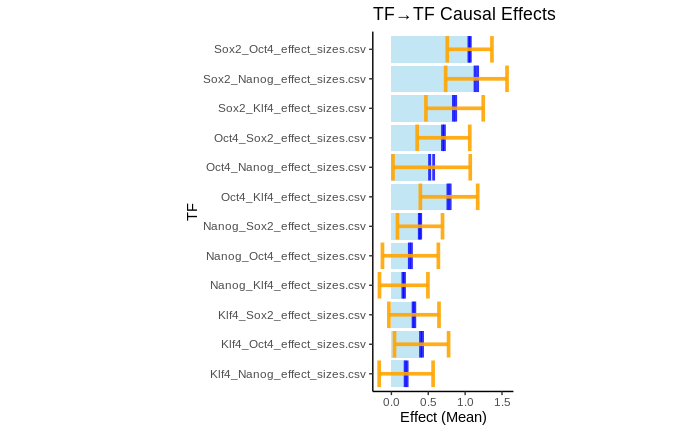
\includegraphics[width=\linewidth]{fig/bpnet_tf_to_tf_global_ces}
		\caption{Global CEs for all pairs of TFs predicted by BPNet. TODO: Annotate with predictions from BPNet paper.}%
		\label{fig:bpnet_tf_to_tf_global_ces}
	\end{subfigure}
	\begin{subfigure}[t]{.5\textwidth}
		\centering
		\includegraphics[width=.4\linewidth]{example-image-a}
		\caption{Example MR plots for 5 sequences and Oct4 \( \rightarrow \) Sox2 and Klf4 \( \rightarrow \) Nanog respectively.}
		\label{fig:bpnet_eff_size_pair_exs}
	\end{subfigure}

	\caption{BPNet results}
\end{figure*}

\paragraph{\method\ correctly identifies which TFs strongly do and do not influence others}%
\label{par:bpnet_res_1}

\subsection{DeepSEA}%
\label{sub:deepsea}
\subsubsection{Setup}%
\label{ssub:deepsea_setup}

\begin{itemize}
	\item Introduce DeepSEA, mention ensemble and calibration method, and dataset / features
	\item Question we were trying to answer: depends on which features we choose to use
\end{itemize}

\section{Discussion}%
\label{sec:discussion}

\subsection{Strengths}%
\label{sub:strengths}
\begin{itemize}
	\item \method\ recovers known patterns in both real model experiments
	\item \method\ can generate new hypothesized relationships for experimental work to investigate
	\item \method's global effect patterns can help validate and improve confidence in models
	\item \method\ is compatible with existing, already trained models 
\end{itemize}

\subsection{Limitations}%
\label{sub:limitations}
\begin{itemize}
	\item Strong assumptions inherited from MR
	\item Quality of estimates depends on model quality
	\item Calibration of CE intervals
	\item Inability to determine correct direction from data
\end{itemize}

\subsection{Future Work}%
\label{sub:future_work}
\begin{itemize}
	\item Network analysis
	\item Bi-directionality \& weakening need for other assumptions
	\item Diagnostics for whether \method\ can be safely applied
\end{itemize}

\section{Conclusion}%
\label{sec:conclusion}
\begin{itemize}
	\item Summarize most important results
	\item Repeat or emphasize framing of deep MR as exciting proof-of-concept for determining what causal relationships multi-task genomic deep learning models learn
	\item (Maybe) connect to larger context/project of trying to make multi-task genomic models more trustworthy
\end{itemize}

\pagebreak
\section{Questions}
\begin{itemize}
	\item What to test with DeepSEA? Options:
	\begin{itemize}
		\item Stick with TFs \( \rightarrow \) accessibility.
		\item PolII occupancy but without doing the promoter enhancer thing?
	\end{itemize}
	\item Should we be using the held-out set as opposed to the training set? In theory, we don't really care about generalization performance so much as just getting the most accurate sense of what the model's learned.
	\item What's our `Theory of change' for the paper?
	\begin{itemize}
		\item Inspire more work in the area
		\item Provide another method for people's toolbox
	\end{itemize}
	\item More separate discussion of local vs.\ global CE quality?
	\item Which MR method?
	\begin{itemize}
		\item Egger has the problem with the intercept going crazy.
		\item MBE seems pretty good for our use-case but is ery slow.
	\end{itemize}
	\item Futz around with z-scores - is it worth it? 
	\item Should we be including heterogeneous effects in the simulation?
\end{itemize}

% Acknowledgements should go at the end, before appendices and references

% Manual newpage inserted to improve layout of sample file - not
% needed in general before appendices/bibliography.

\newpage

\appendix

\vskip 0.2in
\bibliography{bib}

\end{document}

%%% Local Variables:
%%% mode: latex
%%% TeX-master: t
%%% End:
